\chapter{Design}
\label{chap1}

The DLXY is a \texttt{VHDL} implementation of a processor architecture partially
compatible with the DLX architecture described in \textit{Fundamentals of
Computer Design - Patterson, Hennessy}.

\bigskip
DLXY main characteristics include:
\begin{itemize}
	\item RISC Load \& Store architecture
	\item 32-bit data parallelism
	\item bi-endian data encoding
	\item partial DLX instruction set
\end{itemize}

\section{Outside}

\subsection{Interface}
The DLXY core is designed to be inserted in an environment which provides:
\begin{itemize}
	\item the \textbf{clock signal}
	\item some \textbf{configuration signals}
	\item the \textbf{instruction memory}
	\item the \textbf{data memory}
\end{itemize}

\begin{figure}[ht]
	\centering
	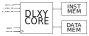
\includegraphics[width=.5\textwidth]{chapters/figures/top_mounted} 
	\caption{The DLXY core inserted in the required environment.}
	\label{fig:env_top}
\end{figure}

\subsubsection{Configuration signals}
When the \textbf{reset signal} is:
\begin{itemize}
	\item not active (low): the processor runs in the "operating mode":
		the execution flows according to the content of the instruction
		memory
	\item active (high): the processor runs in the "configuration mode":
		\begin{itemize}
			\item the internal status is cleared and is set up for
				starting the execution from address 0 of the
				instruction memory
			\item the values of the configuration signals are stored
				and will be used during the operating mode
		\end{itemize}
\end{itemize}

\begin{table}[ht]
	\centering
	\begin{tabular}{ll}
		\hline
		\rowcolor{gray!50}
		Signal & Meaning \\
		ENDIAN & '0': big endian; '1': little endian \\
		\rowcolor{gray!25}
		I\_MEM\_SZ & Size (in lines) of the physical intruction memory 
			(max $2^{32}$) \\
		D\_MEM\_SZ & Size (in lines) of the physical data memory 
			(max $2^{32}$) \\
		\hline
	\end{tabular}
	\label{tab:config_signals}
\end{table}

\subsubsection{Memories}
Both the instruction and the data memory must support asynchronous reading and
must provide the read data within one clock cycle.

The data memory must also provide synchronous writing capabilities.

\bigskip
Table \ref{tab:i_mem_specs} and \ref{tab:d_mem_specs} show the required memory
specifications in detail.

\begin{table}[ht]
	\centering
	\begin{tabular}{llll}
		\hline
		\rowcolor{gray!50}
		Access type & Data size & Address & Timing \\
		Read & Word & Word aligned & Asynchronous \\
		\hline
	\end{tabular}
	\caption{Instruction memory specifications.}
	\label{tab:i_mem_specs}
\end{table}

\begin{table}[ht]
	\centering
	\begin{tabular}{lllll}
		\hline
		\rowcolor{gray!50}
		Access type & Data size & Address & Timing & Control signal \\
		Read & Word & Word aligned & Asynchronous & \texttt{RD = "11"} \\
		\rowcolor{gray!25}
		Read & Half word & Half word aligned & Asynchronous & \texttt{RD = "10"} \\
		Read & Byte & Any & Asynchronous & \texttt{RD = "01"} \\
		\rowcolor{gray!25}
		Write & Word & Word aligned & Synchronous & \texttt{WR = "11"} \\
		Write & Half word & Half word aligned & Synchronous & \texttt{WR = "10"} \\
		\rowcolor{gray!25}
		Write & Byte & Any & Synchronous & \texttt{WR = "01"} \\
		\hline
	\end{tabular}
	\caption{Data memory specifications.}
	\label{tab:d_mem_specs}
\end{table}

\subsection{Instruction set}
The DLXY instruction set is a subset of the original DLX one: it supports all
the instructions involving integers (except for \texttt{LHI}, which can be
easily obtained using the other instructions).

A modified version of \texttt{MULT} instruction between integer half words is
supported too.

\bigskip
Figure \ref{fig:encoding} shows the encoding of each instruction type, while
tables \ref{tab:r_type_inst}, \ref{tab:i_type_inst} and \ref{tab:j_type_inst}
display all the supported instructions.

\begin{figure}[ht]
	\centering
	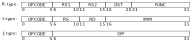
\includegraphics[width=.75\textwidth]{chapters/figures/encoding} 
	\caption{The DLXY instruction encoding.}
	\label{fig:encoding}
\end{figure}

\begin{table}[ht]
	\centering
	\begin{tabular}{ll}
		\hline
		\rowcolor{gray!50}
		Symbol & Result \\
		\texttt{SLL} & \texttt{RF(RD) <= RF(RS1) logic shifted to the left by unsigned(RF(RS2)) bits} \\
		\rowcolor{gray!25}
		\texttt{SRL} & \texttt{RF(RD) <= RF(RS1) logic shifted to the right by unsigned(RF(RS2)) bits} \\
		\texttt{SRA} & \texttt{RF(RD) <= RF(RS1) arithmetic shifted to the right by unsigned(RF(RS2)) bits} \\
		\rowcolor{gray!25}
		\texttt{ADD} & \texttt{RF(RD) <= RF(RS1) + RF(RS2)} \\
		\texttt{ADDU} & \texttt{RF(RD) <= RF(RS1) + RF(RS2)} \\
		\rowcolor{gray!25}
		\texttt{SUB} & \texttt{RF(RD) <= RF(RS1) - RF(RS2)} \\
		\texttt{SUBU} & \texttt{RF(RD) <= RF(RS1) - RF(RS2)} \\
		\rowcolor{gray!25}
		\texttt{MULT} & \texttt{RF(RD) <= low\_half(RF(RS1)) * low\_half(RF(RS2))} \\
		\texttt{AND} & \texttt{RF(RD) <= RF(RS1) AND RF(RS2)} \\
		\rowcolor{gray!25}
		\texttt{OR} & \texttt{RF(RD) <= RF(RS1) OR RF(RS2)} \\
		\texttt{XOR} & \texttt{RF(RD) <= RF(RS1) XOR RF(RS2)} \\
		\rowcolor{gray!25}
		\texttt{SEQ} & \texttt{RF(RD) <= 1 when (RF(RS1) = RF(RS2)) else 0} \\
		\texttt{SNE} & \texttt{RF(RD) <= 1 when (RF(RS1) != RF(RS2)) else 0} \\
		\rowcolor{gray!25}
		\texttt{SLT} & \texttt{RF(RD) <= 1 when (signed(RF(RS1)) < signed(RF(RS2))) else 0} \\
		\texttt{SGT} & \texttt{RF(RD) <= 1 when (signed(RF(RS1)) > signed(RF(RS2))) else 0} \\
		\rowcolor{gray!25}
		\texttt{SLE} & \texttt{RF(RD) <= 1 when (signed(RF(RS1)) <= signed(RF(RS2))) else 0} \\
		\texttt{SGE} & \texttt{RF(RD) <= 1 when (signed(RF(RS1)) >= signed(RF(RS2))) else 0} \\
		\rowcolor{gray!25}
		\texttt{SLTU} & \texttt{RF(RD) <= 1 when (unsigned(RF(RS1)) < unsigned(RF(RS2))) else 0} \\
		\texttt{SGTU} & \texttt{RF(RD) <= 1 when (unsigned(RF(RS1)) > unsigned(RF(RS2))) else 0} \\
		\rowcolor{gray!25}
		\texttt{SLEU} & \texttt{RF(RD) <= 1 when (unsigned(RF(RS1)) <= unsigned(RF(RS2))) else 0} \\
		\texttt{SGEU} & \texttt{RF(RD) <= 1 when (unsigned(RF(RS1)) >= unsigned(RF(RS2))) else 0} \\
		\hline
	\end{tabular}
	\caption{R-type instructions supported by DLXY.}
	\label{tab:r_type_inst}
\end{table}

\begin{table}[ht]
	\centering
	\begin{tabular}{ll}
		\hline
		\rowcolor{gray!50}
		Symbol & Result \\
		\texttt{BEQZ} & \texttt{PC <= (PC + 4 + signed(IMM)) when (RF(RS) = 0) else (PC + 4)} \\
		\rowcolor{gray!25}
		\texttt{BNEZ} & \texttt{PC <= (PC + 4 + signed(IMM)) when (RF(RS) != 0) else (PC + 4)} \\
		\texttt{ADDI} & \texttt{RF(RD) <= RF(RS) + signed(IMM)} \\
		\rowcolor{gray!25}
		\texttt{ADDUI} & \texttt{RF(RD) <= RF(RS) + unsigned(IMM)} \\
		\texttt{SUBI} & \texttt{RF(RD) <= RF(RS) - signed(IMM)} \\
		\rowcolor{gray!25}
		\texttt{SUBUI} & \texttt{RF(RD) <= RF(RS) - unsigned(IMM)} \\
		\texttt{ANDI} & \texttt{RF(RD) <= RF(RS) AND unsigned(IMM)} \\
		\rowcolor{gray!25}
		\texttt{ORI} & \texttt{RF(RD) <= RF(RS) OR unsigned(IMM)} \\
		\texttt{XORI} & \texttt{RF(RD) <= RF(RS) XOR unsigned(IMM)} \\
		\rowcolor{gray!25}
		\texttt{SLLI} & \texttt{RF(RD) <= RF(RS) logic shifted to the left by unsigned(IMM) bits} \\
		\texttt{SRLI} & \texttt{RF(RD) <= RF(RS) logic shifted to the right by unsigned(IMM) bits} \\
		\rowcolor{gray!25}
		\texttt{SRAI} & \texttt{RF(RD) <= RF(RS) arithmetic shifted to the right by unsigned(IMM) bits} \\
		\texttt{SEQI} & \texttt{RF(RD) <= 1 when (RF(RS) = signed(IMM)) else 0} \\
		\rowcolor{gray!25}
		\texttt{SNEI} & \texttt{RF(RD) <= 1 when (RF(RS) != signed(IMM)) else 0} \\
		\texttt{SLTI} & \texttt{RF(RD) <= 1 when (signed(RF(RS)) < signed(IMM)) else 0} \\
		\rowcolor{gray!25}
		\texttt{SGTI} & \texttt{RF(RD) <= 1 when (signed(RF(RS)) > signed(IMM)) else 0} \\
		\texttt{SLEI} & \texttt{RF(RD) <= 1 when (signed(RF(RS)) <= signed(IMM)) else 0} \\
		\rowcolor{gray!25}
		\texttt{SGEI} & \texttt{RF(RD) <= 1 when (signed(RF(RS)) >= signed(IMM)) else 0} \\
		\texttt{SLTUI} & \texttt{RF(RD) <= 1 when (unsigned(RF(RS)) < unsigned(IMM)) else 0} \\
		\rowcolor{gray!25}
		\texttt{SGTUI} & \texttt{RF(RD) <= 1 when (unsigned(RF(RS)) > unsigned(IMM)) else 0} \\
		\texttt{SLEUI} & \texttt{RF(RD) <= 1 when (unsigned(RF(RS)) <= unsigned(IMM)) else 0} \\
		\rowcolor{gray!25}
		\texttt{SGEUI} & \texttt{RF(RD) <= 1 when (unsigned(RF(RS)) >= unsigned(IMM)) else 0} \\
		\texttt{LB} & \texttt{RF(RD) <= signed(low\_byte(MEM(RF(RS) + signed(IMM))))} \\
		\rowcolor{gray!25}
		\texttt{LH} & \texttt{RF(RD) <= signed(low\_half(MEM(RF(RS) + signed(IMM))))} \\
		\texttt{LW} & \texttt{RF(RD) <= MEM(RF(RS) + signed(IMM))} \\
		\rowcolor{gray!25}
		\texttt{LBU} & \texttt{RF(RD) <= unsigned(low\_byte(MEM(RF(RS) + signed(IMM))))} \\
		\texttt{LHU} & \texttt{RF(RD) <= unsigned(low\_half(MEM(RF(RS) + signed(IMM))))} \\
		\rowcolor{gray!25}
		\texttt{SB} & \texttt{MEM(RF(RS) + signed(IMM)) <= low\_byte(RF(RD))} \\
		\texttt{SH} & \texttt{MEM(RF(RS) + signed(IMM)) <= low\_half(RF(RD))} \\
		\rowcolor{gray!25}
		\texttt{SW} & \texttt{MEM(RF(RS) + signed(IMM)) <= RF(RD)} \\
		\texttt{NOP} & Null \\
		\hline
	\end{tabular}
	\caption{I-type instructions supported by DLXY.}
	\label{tab:i_type_inst}
\end{table}

\begin{table}[ht]
	\centering
	\begin{tabular}{ll}
		\hline
		\rowcolor{gray!50}
		Symbol & Result \\
		\texttt{J} & \texttt{PC <= PC + 4 + signed(OFF)} \\
		\rowcolor{gray!25}
		\texttt{JAL} & \texttt{PC <= PC + 4 + signed(OFF); R31 <= PC + 4} \\
		\texttt{JR} & \texttt{PC <= RF(RS)} \\
		\rowcolor{gray!25}
		\texttt{JALR} & \texttt{PC <= RF(RS); R31 <= PC + 4} \\
		\hline
	\end{tabular}
	\caption{J-type instructions supported by DLXY.}
	\label{tab:j_type_inst}
\end{table}

\section{Architecture}
The DLXY core is made up of two components: an hardwired \textbf{control unit}
and a pipelined \textbf{datapath}.

\subsection{Datapath}

\subsection{Control unit}
The DLXY control unit is the component in charge of translating the code
of the instruction in the \textbf{decode stage} into control signals
needed by the datapath to correctly execute the instruction.

\bigskip
The control unit work consists in two main subtasks:
\begin{itemize}
	\item \textbf{instruction decoding}: translate instruction code into
		control signals, regardless of the processor status
	\item \textbf{hazard management}: ensure the correct instruction result,
		depending on the other instructions being executed in the pipeline
\end{itemize}

\subsubsection{Hazard management}

\paragraph{Control hazards} \mbox{} \\
A control hazard happens whenever a \textbf{branch is taken}: since the control
unit operates during the decode stage, while the branch is detected, the 
instruction stored at the address following the current one's is fetched, as if
there wasn't any branch.

In order to solve this issue, \textbf{forces a \texttt{NOP}} to the instruction
following a taken branch, since it could possibly bring the processor to an
incorrect state.

\bigskip
If a conditional branch is not taken the execution can proceed without any
penalty to pay: this technique is called \textbf{static untaken branch prediction}.

\paragraph{Data hazards} \mbox{} \\
In an in-order pipeline the only possible data hazard is the \textbf{Read After
Write} hazard, which occurs when an instruction $I_A$ source operand matches
another instruction $I_B$ destination operand and $I_A$ enters the pipeline
before $I_B$ exits it.

\bigskip
The DLXY solves these hazards in two ways:
\begin{itemize}
	\item \textbf{data forwarding}:
	\item \textbf{stall insertion}:
\end{itemize}

\subsubsection{Design style considerations}
An \textbf{hardwired} control unit is an ad-hoc combinational circuit:
this design style allows \underline{better performance} and \underline{lower power}
consumption with respect to other styles, such as microprogrammed control units,
at the expense of a \underline{lower mantainability}.

\bigskip
Since the DLXY is quite a simple core, the hardwired design style had been the
natural choice.

\section{Circuit}

